\section{Results}

	\begin{center}
	\begin{tabular}{ l | c | r }
		\hline
		Parameters & Values $A, B$ & Description \\ \hline
		L & $7.5$ & Length half size demain  \\ 
		R & ? &  radius \\
	
		$\mu$ & 1  & ..\\
		$\nu_c$  & .&  . \\
		$\nu_d$  & .&  . \\
		k & . & .\\
		D & & \\
		$\beta$ & & \\
		$\delta$ & & \\
		%	$N_A$ & 250 & particles of type A\\
%	$N_B$ & 250 & particles of type B \\
		\hline
	\end{tabular}
\end{center}	




%----------PLOTS
% DO NOT DELETE - NE PAS EFFACHER ---------------------
%\begin{figure}
%	\centering
%	\begin{minipage}[h]{%0.5\linewidth}
%	\centering
%	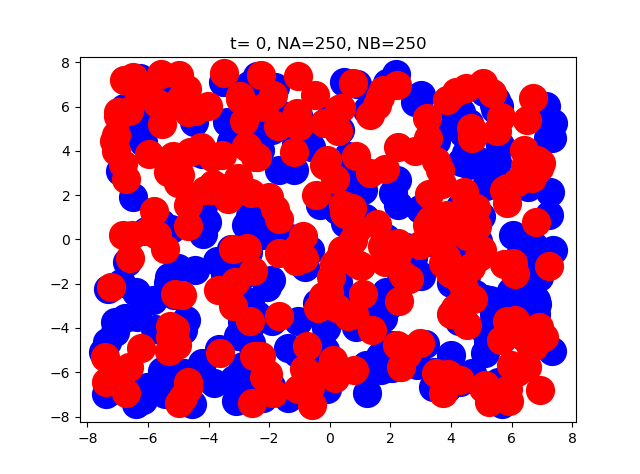
\includegraphics[width=1\linewidth]{micro_ini_caseI1}
%	%\captionof{figure}{ }\label{fig:1}
%	\end{minipage}
%\hfill
%	\begin{minipage}[h]{%0.5\linewidth}
%	\centering
%	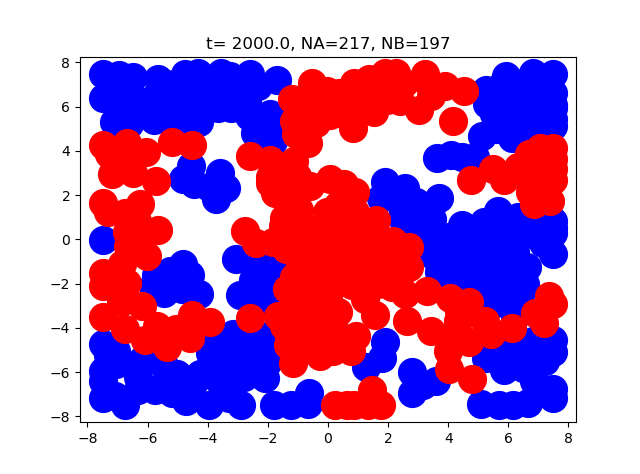
\includegraphics[width=1\linewidth]{micro_fin_caseI1}
%	%\captionof{figure}{ }\label{fig:2}
%	
%%{case I: A-cells blue, B-cells red with $k^{AA}=k^{BB}=2 $, $k^{AB}=k^{BA}=8$; $b0_A=b0_B=10^{-3}$, $d0_A=d0_B=7\cdot10^{-4}$}	
%	\end{minipage}
%\end{figure}
%-----------------------------------------------------

% DO NOT DELETE - NE PAS EFFACHER
%2: {case I: A-cells blue, B-cells red with $k^{AA}=k^{BB}=2 $, $k^{AB}=k^{BA}=8$; $b0_A=b0_B=2\cdot10^{-3}$, $d0_A=d0_B=7\cdot10^{-4}$}

%3: {case I: A-cells blue, B-cells red with $k^{AA}=k^{BB}=2 $, $k^{AB}=k^{BA}=8$; $b0_A=b0_B=10^{-4}$, $d0_A=d0_B=7\cdot10^{-5}, \th_A=\th_B=8\cdot 10^{-5}$}

%4: {case I: A-cells blue, B-cells red with $k^{AA}=k^{BB}=2 $, $k^{AB}=k^{BA}=4$; $b0_A=b0_B=10^{-4}$, $d0_A=d0_B=7\cdot10^{-5}, \th_A=\th_B=8\cdot 10^{-5}$}

%5: {case I: A-cells blue, B-cells red with $k^{AA}=k^{BB}=2 $, $k^{AB}=k^{BA}=2$; $b0_A=b0_B=10^{-4}$, $d0_A=d0_B=10^{-5}, \th_A=\th_B=8\cdot 10^{-5}$}

%6: {case I: A-cells blue, B-cells red with $k^{AA}=k^{BB}=2 $, $k^{AB}=k^{BA}=2$; $b0_A=b0_B=10^{-4}$, $d0_A=d0_B=10^{-5}, \th_A=\th_B=8\cdot 10^{-5}$}



\begin{figure}[htb]
	\begin{minipage}[t]{.45\textwidth}
		\centering
		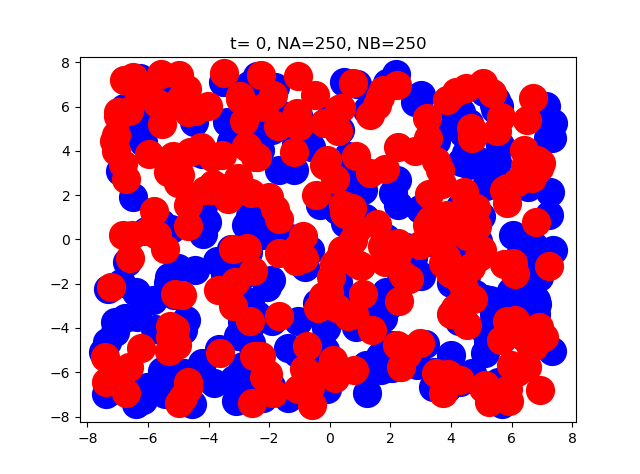
\includegraphics[width=\textwidth]{micro_ini_caseI1}
	%	\subcaption{Image 1.}\label{fig:1}
	\end{minipage}
	\hfill
	\begin{minipage}[t]{.45\textwidth}
		\centering
		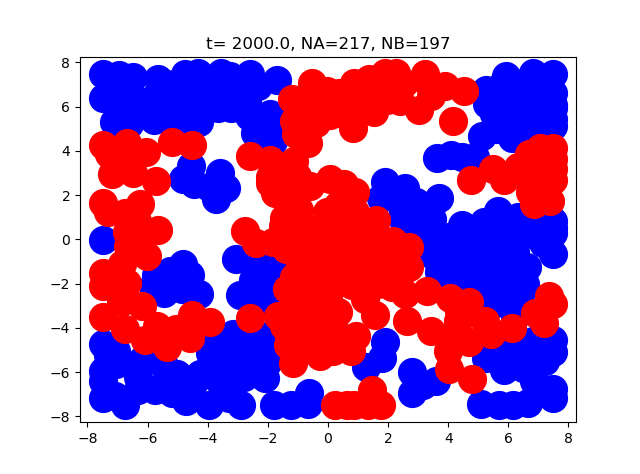
\includegraphics[width=\textwidth]{micro_fin_caseI1}
	%	\subcaption{Image 2.}\label{fig:2}
	\end{minipage}  
	\label{fig:1-2}
	\caption{{case I: A-cells blue, B-cells red with $k^{AA}=k^{BB}=2 $, $k^{AB}=k^{BA}=8$; $b0_A=b0_B=10^{-3}$, $d0_A=d0_B=7\cdot10^{-4}$}, $\th_A=\th_B=8\cdot 10^{-4}$}
\end{figure}


\begin{figure}[htb]
	\begin{minipage}[t]{.45\textwidth}
		\centering
		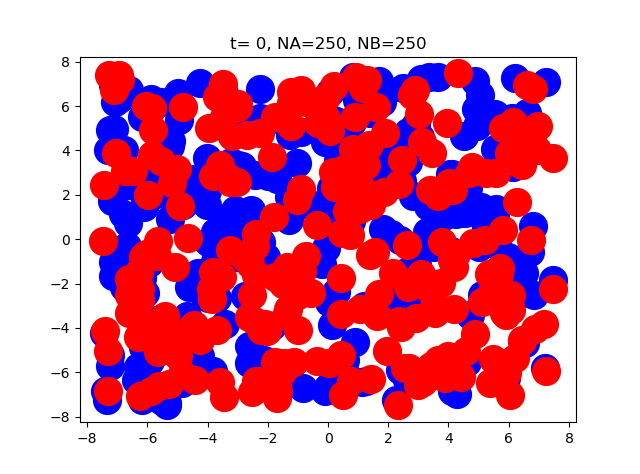
\includegraphics[width=\textwidth]{micro_caseI_ini2}
		%	\subcaption{Image 1.}\label{fig:1}
	\end{minipage}
	\hfill
	\begin{minipage}[t]{.45\textwidth}
		\centering
		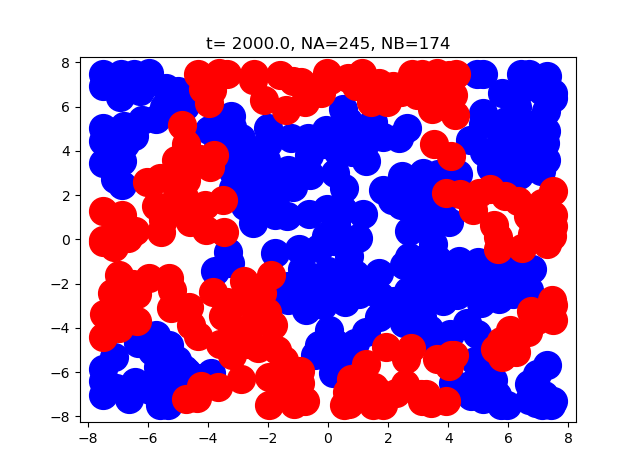
\includegraphics[width=\textwidth]{micro_caseI_fin2}
		%	\subcaption{Image 2.}\label{fig:2}
	\end{minipage}  
	\label{fig:1-2}
	\caption{{case I: A-cells blue, B-cells red with $k^{AA}=k^{BB}=2 $, $k^{AB}=k^{BA}=8$; $b0_A=b0_B=2\cdot10^{-3}$, $d0_A=d0_B=7\cdot10^{-4}$, $\th_A=\th_B=8\cdot 10^{-4}$}	}
\end{figure}


\begin{figure}[htb]
	\begin{minipage}[t]{.45\textwidth}
		\centering
		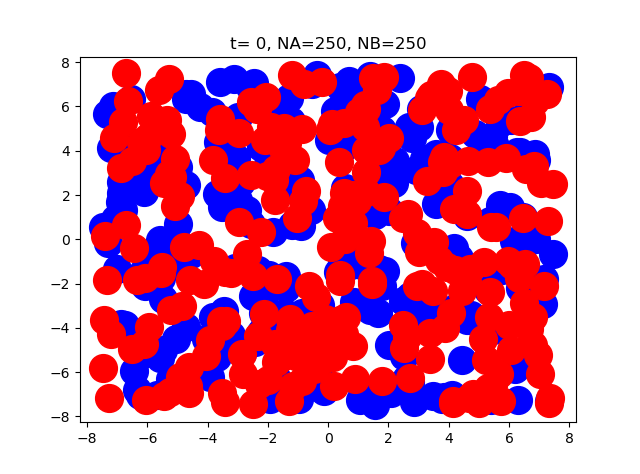
\includegraphics[width=\textwidth]{micro_caseI_ini3}
		%	\subcaption{Image 1.}\label{fig:1}
	\end{minipage}
	\hfill
	\begin{minipage}[t]{.45\textwidth}
		\centering
		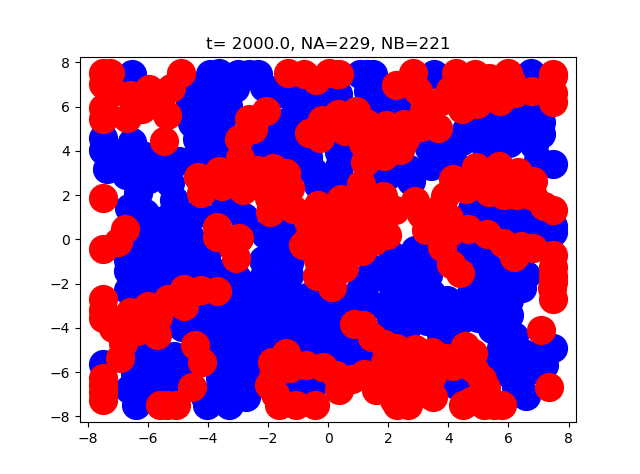
\includegraphics[width=\textwidth]{micro_caseI_fin3}
		%	\subcaption{Image 2.}\label{fig:2}
	\end{minipage}  
	\label{fig:1-2}
	\caption{{case I: A-cells blue, B-cells red with $k^{AA}=k^{BB}=2 $, $k^{AB}=k^{BA}=8$; $b0_A=b0_B=10^{-4}$, $d0_A=d0_B=7\cdot10^{-5}, \th_A=\th_B=8\cdot 10^{-5}$}	}
\end{figure}



\begin{figure}[htb]
	\begin{minipage}[t]{.45\textwidth}
		\centering
		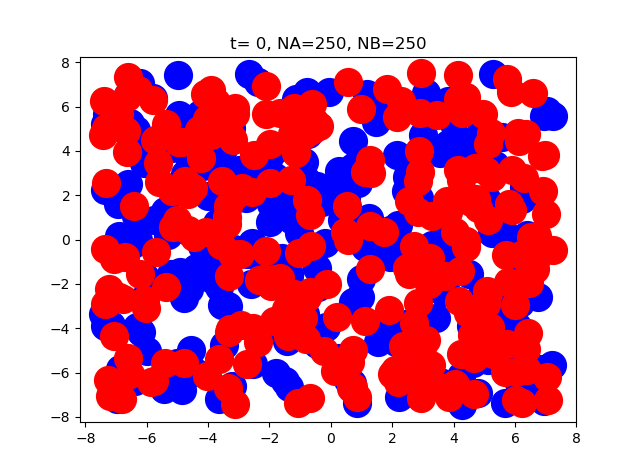
\includegraphics[width=\textwidth]{micro_caseI_ini4}
		%	\subcaption{Image 1.}\label{fig:1}
	\end{minipage}
	\hfill
	\begin{minipage}[t]{.45\textwidth}
		\centering
		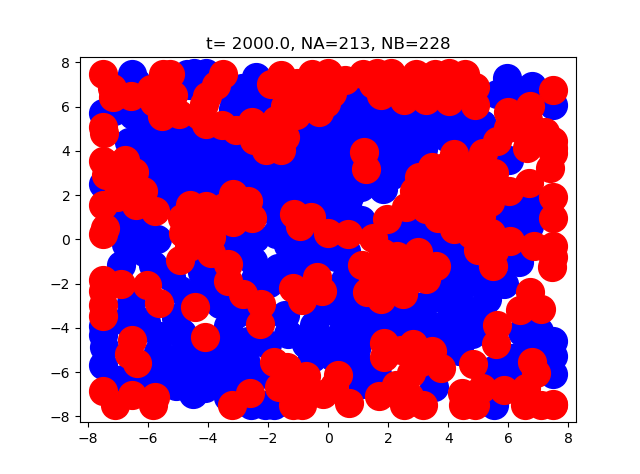
\includegraphics[width=\textwidth]{micro_caseI_fin4}
		%	\subcaption{Image 2.}\label{fig:2}
	\end{minipage}  
	\label{fig:1-2}
	\caption{{case I: A-cells blue, B-cells red with $k^{AA}=k^{BB}=2 $, $k^{AB}=k^{BA}=4$; $b0_A=b0_B=10^{-4}$, $d0_A=d0_B=7\cdot10^{-5}, \th_A=\th_B=8\cdot 10^{-5}$}	}
\end{figure}


\begin{figure}[htb]
	\begin{minipage}[t]{.45\textwidth}
		\centering
		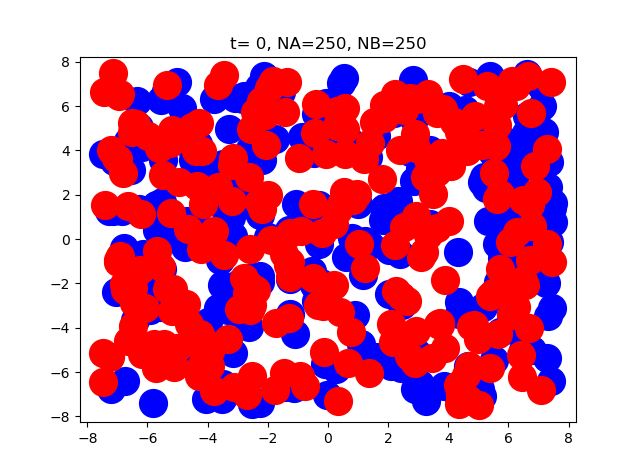
\includegraphics[width=\textwidth]{micro_caseI_ini5}
		%	\subcaption{Image 1.}\label{fig:1}
	\end{minipage}
	\hfill
	\begin{minipage}[t]{.45\textwidth}
		\centering
		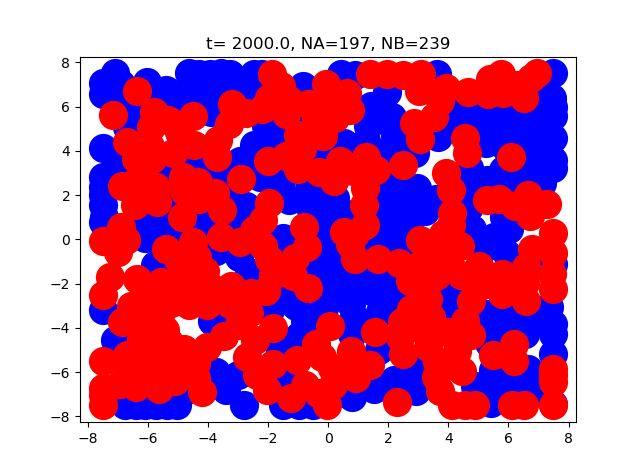
\includegraphics[width=\textwidth]{micro_caseI_fin5}
		%	\subcaption{Image 2.}\label{fig:2}
	\end{minipage}  
	\label{fig:1-2}
	\caption{{case I: A-cells blue, B-cells red with $k^{AA}=k^{BB}=2 $, $k^{AB}=k^{BA}=2$; $b0_A=b0_B=10^{-4}$, $d0_A=d0_B=10^{-5}, \th_A=\th_B=8\cdot 10^{-5}$}}
\end{figure}



%\begin{figure}[htb]
%	\begin{minipage}[t]{.45\textwidth}
%		\centering
%		\includegraphics[width=\textwidth]{micro_caseI_ini6}
%		%	\subcaption{Image 1.}\label{fig:1}
%	\end{minipage}
%	\hfill
%	\begin{minipage}[t]{.45\textwidth}
%		\centering
%		\includegraphics[width=\textwidth]{micro_caseI_fin6}
%		%	\subcaption{Image 2.}\label{fig:2}
%	\end{minipage}  
%	\label{fig:1-2}
%	\caption{{case I: A-cells blue, B-cells red with $k^{AA}=k^{BB}=2 $, $k^{AB}=1.38, k^{BA}=2\cdot k^{AB}$; $b0_A=b0_B=10^{-4}$, $d0_A=d0_B=10^{-5}, \th_A=\th_B=8\cdot 10^{-5}$}}
%\end{figure}




